%==============================================================================
\documentclass[11pt,oneside,onecolumn,letterpaper]{article}
\usepackage{times}
\usepackage[paperwidth=8.5in, paperheight=11in,
top=2.5cm, bottom=2.6cm, left=2.58cm, right=2.53cm]{geometry}
%\setlength{\textheight} {9.00in}
%\setlength{\textwidth}  {6.40in}
%\setlength{\topmargin}  {-0.50in}
%%\setlength{\headheight} {0.00in}
%%\setlength{\headsep}     {0.40in}
%\setlength{\oddsidemargin}{-0.010in}
%\setlength{\evensidemargin}{-0.00in}
%==============================================================================
%\usepackage{algorithm}
\usepackage{amssymb}
\usepackage{color}
\usepackage{booktabs}
\usepackage{graphicx}
\usepackage{latexsym}
\usepackage{subfigure}
\usepackage{wrapfig}
\usepackage{amsmath}
\usepackage{amsthm}
\usepackage[hyphens]{url}
\usepackage{pifont}
\usepackage{color}
\usepackage{colortbl}
\usepackage[lined, boxed, linesnumbered]{algorithm2e}
\usepackage[square, comma, sort&compress, numbers]{natbib}

\newcounter{alg}
\newenvironment{enum-ref}{
\begin{list}%
{[\arabic{alg}]} {\usecounter{alg}
  \setlength{\leftmargin} {0.25in}
  \setlength{\labelwidth} {0.30in}
  \setlength{\rightmargin}{0.00in}
  \setlength{\topsep}     {0.00in}}
}{\end{list}}

\newenvironment{enum-number}{
\begin{list}%
{\arabic{alg})} {\usecounter{alg}
  \setlength{\leftmargin} {0.25in}
  \setlength{\labelwidth} {0.30in}
  \setlength{\rightmargin}{0.00in}
  \setlength{\topsep}     {0.00in}}
}{\end{list}}

\newenvironment{enum-nonum}{
\begin{list}%
{$\bullet$} {
  \setlength{\leftmargin} {0.25in}
  \setlength{\labelwidth} {0.30in}
  \setlength{\rightmargin}{0.00in}
  \setlength{\topsep}     {0.00in}}
}{\end{list}}

\let\chapter\section

%==============================================================================
\pagestyle{plain}
%==============================================================================

\title{Secure Avionics Flight Firmware Installation Routine System Design}
\author{MITRE eCTF 2022\\Team \textbf{Cacti}\\ University at Buffalo}
\date{}



\begin{document}
%%
%=============================================================================
\normalsize


\maketitle
%\date{}

\renewcommand{\thepage}{System Design, Team Cacti, University at Buffalo--\arabic{page}}
\setcounter{page}{1} \normalsize
%
%\renewcommand{\baselinestretch}{1.2}
%\normalsize
%\vspace{0.1in}
%\centerline{\textbf{\Large }}
%\renewcommand{\baselinestretch}{1.0}
%\normalsize

\newcommand{\flagRollback}{\textsf{Rollback}\xspace}

\section{Introduction}

This section presents the entities and communication channels in the system.

\subsection{Entities}

The following summarizes the entities in the system.

\begin{itemize}
  \item Host is a general-purpose computer in the secure facility, which is responsible for generating protected firmware and configuration data images.
	\item A SAFFIRE bootloader is the main entity of the system to ensure the secure loading of flight configuration data and firmware with version updates on the device.
	It receives commands from the host to boot the firmware, put firmware on SRAM and handover the execution. 
	Moreover, the bootloader is also responsible for providing a readback feature of the firmware and configuration data to an authenticated host.
	\item The firmware in the avionic device contains the logic to control the flight. 
	The firmware gets the flight itinerary from the configuration files.
	As the flight travel is dependent on this logic and data the bootloader needs to ensure that no malicious code or data is loaded on the device.
  \item  EEPROM on the Tivaware device is a hardware component accessible to the bootloader, which can be used to store data with access permissions.
\end{itemize}

\section{Attack Models}

The attackers can carry out the following attacks:

\begin{itemize}
  \item Attackers may install custom or modified firmware and configurations, and compromise the flight.
  \item Attackers may install old and buggy version of the firmware.
  \item Attackers may access host secrets.
  \item Side-channel attack.
  \item Hardware trojan.
\end{itemize}


\section{Our Design}

The host $H$ has its private key $sk_k$ stored in the host secrets file.
The bootloader can access the associated public key $pk_k$ and three AES256-GCM keys for firmware ($k_f$), configuration ($k_c$), and version number ($k_v$) protection, which are stored in the EEPROM.
EEPROM also stores additional data or secrets that the bootloader needs at run-time.
To protect the EEPROM we utilize EEPROM block hiding feature.

MPU is configured to 1) prevent the EEPROM from being accessed by an invalid host; 2) set the FLASH as eXecute-Never (XN) except for the bootloader, 3) set the FLASH as read and write (RW) for the bootloader only. 

ENC and DEC stand for symmetric encryption and decryption with AES256-GCM.
AENC and ADEC stand for asymmetric encryption and decryption with RSA512.
SIG and AUTH stand for the signature and verification with RSA512.

\subsection{Key Protection}
The asymmetric $pk_k$, symmetric $k_f$, $k_c$, and $k_v$ are kept in the EEPROM region memory for the bootloader to access at run-time.
When the bootloader starts execution it configures the MPU, which allows only the bootloader itself to access the EEPROM memory.
After that, it copies the keys from the EEPROM to the flash memory.
Immediately, EEPROM blocks containing the keys are locked using the EEPROM block locking feature, which denies read/write access for everyone until reset.
Thus, even if attackers can overwrite the MPU configurations, they can not access the EEPROM memory.

\subsection{Firmware and Configuration Data Protection}
Symmetric crypto is used for firmware, configuration data, version number protection, $k_f$, $k_c$, and $k_v$.
Our developed host tools implement two layers of symmetric encryption, the outer layer is to protect the authenticity, integrity of the version number and the inner layer for the firmware body.
We keep the firmware and configuration data in encrypted form in flash memory, whereas at firmware boot time we put the decrypted firmware in SRAM and decrypt the configuration data in flash.
Figure~\ref{fig:frmt} demonstrates the format of protected images.

\begin{figure}[!htbp]
	\begin{centering}
		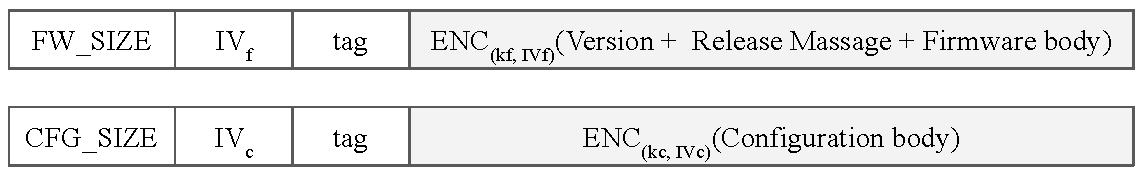
\includegraphics[width = .80\textwidth]{pic/FW_CFG_FORMAT.pdf}
		\caption{Protected Firmware and Configuration Format}
		\label{fig:frmt}
	\end{centering}
\end{figure}

\subsubsection{Host tools}
Our host tools first use firmware encryption key $k_f$ and $IV$ encrypt the firmware binary and release message: ($\mathcal{C}_{FW}$, $tag_f$) = ENC$_{k_f, iv}$(Firmware Body + Release Message).
Then we use the version encryption key $k_v$ and $IV$ to encrypt the version number and $tag_f$: ($\mathcal{C}_V$, $tag_v$) = ENC$_{k_v, iv}$($\mathcal{V} + tag_f$).
The finalized protected firmware contains firmware size, IV and $tag_v$ as the header and $\mathcal{C}_V$ and $\mathcal{C}_{FW}$ as the body.

Similar to protect the firmware, host tools use configuration key $k_c$ and $IV_c$ to encrypt the configuration: ($\mathcal{C}_{CFG}$, $tag_c$) = ENC$_{k_c, iv_c}$(Configuration Body).
Then the protected configuration has configuration size, $IV_c$ and $tag_c$ as the header and $\mathcal{C}_{CFG}$ as the body.

\subsubsection{Bootloader}

\textbf{Update}: 

\textit{Firmware version checking}:
Whenever the bootloader receives the update firmware command, it uses the $IV$ and the symmetric key $k_v$ to decrypt the $C_V$: ($\mathcal{V}'$, $tag_v'$, $tag_f'$) = DEC$_{k_v, iv}(\mathcal{C}_V)$).
If $tag_v'$ matches $tag_v$, it passes version integrity checking.
Then it validates the version number with the previously installed one to decide whether accept or reject this update.
If valid, bootloader keeps the tag $tag_f'$, $IV$ and firmware size to check the firmware integrity.

\textit{Firmware integrity checking}:
After validating the version number, bootloader uses $IV$ and the symmetric key $k_f$ to decrypt the $\mathcal{C}_{FW}$: ($\mathcal{P}$, $tag_f'$) = DEC$_{k_f, iv}(\mathcal{C}_{FW})$).
If $tag_f'$ matches $tag_f$, it passes firmware integrity checking.
Then bootloader updates the encrypted firmware ($\mathcal{C}_{FW}$) in flash memory.
Otherwise, the update will be rejected.

\textit{Configuration integrity checking}.
Whenever the bootloader receives the update firmware command.
The process is similar to firmware integrity checking.

\textbf{Boot firmware}: 
At firmware boot time the bootloader decrypts the firmware body and release message with key $k_f$ and $IV$ ($FW_{body}, Rel_{msg}, tag'_f$ = DEC$_{k_v, iv}(C_{FW})$).
The tags $tag'_f$ and $tag_f$ are compared for integrity checking.
On successful verification the bootloader puts the firmware plaintext in SRAM.

The configuration data is handled the same way as the firmware with one layer of symmetric crypto with key $k_c$ and $IV_c$.

\subsection{Prevent Version Rollback}
Bootloader maintains the version number of firmware in flash memory with MPU configuration.
The version number is part of the encrypted body in the protected firmware binary.
Only the newer, equal, or zero version of the firmware can be installed.

\subsection{Readback Host Authentication}
Asymmetric crypto is for readback functionality, the host generates a public key pair ($pk_k, sk_k$).
The secret key $sk_k$ never leaves the host, while the public key $pk_k$ is loaded on the devices as EEPROM data.
We implement a digital signature mechanism to ensure that only the valid host can request a readback.
\begin{itemize}
  \item[Step 1.] Initialize readback function. 
  The host (or attacker) sends the command \textbf{R} through UART to bootloader.
  Bootloader initiates readback and waits for the authentication message.  
  \item[Step 2.] Host sends authentication message.
  The host generates a digest ($\mathcal{P_H}$), which is a random plaintext ($\mathcal{P}$) hashed by SHA-256.
  Then it uses the private key $sk_k$ to encrypt the digest, $\mathcal{C}$ = ENC$_{sk_k}(\mathcal{P_H})$.
  The ciphertext $\mathcal{C}$ \& plaintext $\mathcal{P}$ will be sent through UART to the bootloader ($\mathcal{C}$, $\mathcal{P}$).
  \item[Step 3.] Bootloader authenticates the host.
  The bootloader uses the associated public key $pk_k$ from EEPROM to decrypt the ciphertext and get the message digest $\mathcal{P_H}$ = DEC$_{pk_k}(\mathcal{C})$.
  Lastly, it generates a second messages digest $\mathcal{P'_H}$ directly from the received plaintext $\mathcal{P}$ and compares both digests $\mathcal{P'_H}$.
  If they do not match, discard.
  Otherwise: response the readback request.
  
  \item [Step 4.] Decrypt the requested memory of the firmware or configuration data and write response on the UART connection for the host.
\end{itemize}

% \subsection{Defeat Hardware Trojan}

% \subsection{Defeat Side-channel Attacks}

% \subsection{Build Process}

%   Describe the important changes in build process.

% \section{Implementation}
% \subsection{Critical Functions and Files}


% \section{Flag Protection}

% \subsection{\textsf{D}}


\end{document}
%==============================================================================
